\section{Vortex Dynamics in a Turbulent Mixing Layer}
\label{sect:velocity}
Analysis of the evolution, interaction, and disintegration of the large-scale structures, and ultimately the noise generated thereby, is greatly simplified by the acquisition of time-resolved flow-field measurements.
Furthermore, as will be explained in \sect{sect:source}, computation of the aeroacoustic source field from a simplified acoustic analogy will require time-resolved flow-field data.
Unfortunately, directly acquiring time-resolved velocity fields for the jet currently under study is simply not possible due to the combination of a large domain of interest ($0 \leq x/D \lesssim 12, 0 \leq r/D \lesssim 3$) and high characteristic frequencies on the order of tens of kHz.
Full-field, high-fidelity measurement techniques capable of this required repetition rate were not available to the researchers.
An indirect method is therefore required in order to estimate the evolution of the large-scale structures, in a reduced-order sense.

Phase-locking of a data acquisition system to a reference signal (such as an actuator or a naturally occurring resonance tone) is a common experimental technique, and was initially considered for the present work.
However, sample analysis performed using a numerical database indicated that a very high temporal resolution was required in order to accurately compute fluctuation rates in the dilatation field (the relevance of which will become more apparent in the following section).
At moderate to high excitation frequencies, this was feasible, though potentially tedious (for example, $\sim$16 phases were estimated as necessary at $St_{DF} =0.25$).
At $St_{DF} =0.05$ however, this would require roughly \textit{forty} phases (the significant dead time between actuations means that it is not necessary to acquire the entire range of phases from $0$ to $2\pi$, but this is small consolation).
Clearly, a more efficient data acquisition method is needed.

\subsection{Stochastic Estimation}
The current work borrows heavily from the methodology of \citet{Tinney2008b} and \citet{Sinha2010} in order to estimate the two-component time-resolved velocity field on a streamwise slice of the jet.
The computational methodology by which the stochastic estimation is performed has been modified, however.
Complementary stochastic estimation is used, due to its significantly lower computational cost as well as theorized improvement in accuracy \citep{Bonnet1994}.
The estimated velocity fields produced by LSE were projected onto the POD eigenfunctions (computed from the random, non-time-resolved velocity fields) to produce an estimate of the time-dependent POD coefficients, which can then be used to reconstruct low-order representations of the estimated random velocity field.
Multiple time delays are incorporated, as this has been found to significantly improve the accuracy of the reconstructions for many flow regimes \citep{Ewing1997,Tinney2006,Tinney2008b,Durgesh2010}.
Instead of performing the stochastic estimation using either linear or higher-order cross-correlations (or cross-spectra), the conditional mapping between the near-field pressure and the POD modal coefficients will be generated by an artificial neural network (ANN).
ANNs were chosen over the more traditional cross-correlations due to their simplicity compared to high-order methods as well as their demonstrated ability to model nonlinear processes in turbulent flows \citep{Lasagna2015}.

A feedforward network structure was used; it was comprised of an input layer, to which near-field pressure traces were supplied, a single hidden layer containing 32 neurons, and an output layer which produced estimates of the time-varying POD coefficients. 
The hidden and output layers were fully connected, and the modified logistic function (hyperbolic tangent) was used as the activation function.
The pressure traces were centered around the acquisition of a PIV image group, and were downsampled to 100 kHz in order to approximate the frequency response of the microphones.
The record time supplied for each training block was $\pm 2.56$ milliseconds; this was determined by estimating the time delay for a large-scale structure to convect through the experimental domain (the convective velocity of the large-scale structures was conservatively estimated as $U_c \simeq 0.5 U_j$).

POD modes and time-varying coefficients were computed from the velocity fields using the method of snapshots \citep{Sirovich1987}; the kernel was defined as the two-component turbulent kinetic energy.
The instantaneous velocity fields were not preprocessed prior to the decomposition (that is, missing or spurious vectors were not replaced or interpolated).
As experimental noise in the velocity fields will be completely uncorrelated to the near-field measurements, it will be filtered out by the stochastic estimation and hence preprocessing is unnecessary.
In this work, the coefficients for every POD mode were estimated, rather than just the most energetic modes, for two reasons.
First, it is not guaranteed that an individual POD mode corresponds to a physically distinct turbulent flow structure or event - an event may be broken up into multiple POD modes of varying energy levels.
Secondly, the most energetic POD mode is not necessarily the most relevant mode for the acoustic generation process (see \citet{Jordan2007} for a modification to the standard POD kernel in order to mitigate this issue).
The second issue is in fact not unique to the field of aeroacoustics but vexes turbulence research in general, where highly relevant dynamical processes may contain little energy \citep{Noack2008}; this has lead researchers to propose alternative methods for extracting dynamical features of turbulent flows \citep{Schmid2010}.
Even though the network is estimating even the least-energetic modes, the current method is far more computationally efficient than directly estimating the velocity fields themselves.

Learning was accomplished via the standard backpropagation method \citep{Haykin1994}, which approximates the error surface of the cost function using first-order derivatives; the error `propagates' backwards from the output neurons to the hidden neurons and the synaptic weights at each neuron are updated to identify the (hopefully, global) minimum of the cost function using gradient descent.
The cost function was defined as the mean-squared-error between the predicted and measured expansion coefficients for a given PIV image group.
Training of the network was performed using the roughly 1500 ensemble pressure-velocity blocks of data (a few PIV images in each set had to be discarded due to laser misfires); synaptic weights were updated based on the average of all blocks (batch processing) using a constant learning rate.
In order to prevent over-fitting, the training was limited to 5000 epochs; $L_1$ regularization was also investigated and found to produce similar results.
A well-known issue with the gradient descent optimization method is that it has a tendency to get trapped in local minima and fails to converge to the global minimum.
Therefore, sample results were also calculated using a much different learning algorithm: adaptive particle swarm optimization.
Details will not be presented here however, as the results were found to not differ substantially from those produced by the backpropagation algorithm (while requiring significantly higher computational resources).


\subsection{Large-Scale Structure Disintegration}
\citet{Hileman2005} investigated the evolution and interactions of large-scale structures and ultimately how these relate to the noise generation process in a supersonic, ideally-expanded jet by combining time-resolved flow visualizations with a three-dimensional microphone array.
Their results showed that the dominant noise was being generated near the end of the potential core, in the region where the shear layers merged.
Large-amplitude, highly-intermittent acoustic events were found to be associated with a fluctuation in the length of the potential core, which the authors ultimately speculated was related to the passage and finally the rapid disintegration of large-scale coherent structures just downstream of the end of the potential core.
The dynamics of the large-scale structures in this region, namely the structure disintegration, are therefore of particular concern to the current work.

Vortex identification was performed by computing the swirling strength at each instance in the estimated velocity field; details and justification for this method can be found in \citet{Adrian2000}.
The evolution of the impulsively excited ($St_{DF} = 0.05$) vortex ring has been tracked in \fig{fig:ch4_impulse_structure_disintegration}.
For ease of visualization, a two-dimensional, five-point boxcar filter was applied to the estimated velocity fields prior to computing the swirling strength, and the results have been phase-averaged based on the recorded LAFPA trigger signal over roughly 30 excitation periods.
Lastly, a solid red line has been overlain to approximately match the convective velocity of the structures.
Only a select number of phases are shown here, as a significant amount of dead time between excitations occurs due to the mismatch in the spatial and temporal characteristic frequencies of the large-scale structures.
\begin{figure}
	\centering
	\includegraphics[width=4in]{Figures/ch4_St005_lambda.png}
	\caption{Evolution of the independent vortex ring ($St_{DF}=0.05$), as visualized using swirling strength. Images are shown at constant phase steps of roughly $\pi/8$, starting with a phase of $\pi/4$.}
	\label{fig:ch4_impulse_structure_disintegration}
\end{figure}

As already known from prior experiments at the GDTL \citep{Kearney-Fischer2009}, the excitation produces a strong roll-up of vortical (toroidal) fluid in the near-nozzle region; in the present case the large-scale structure generated by the excitation is clearly discernible over the background turbulence (and experimental/computational noise) by $x/D \simeq 1$.
The rapid growth of the vortex slows by $x/D \simeq 1.5$ and it advects downstream relatively unchanged until  $x/D \simeq 4$.
It is at this point that the vortex undergoes a rapid disintegration, yielding smaller scale, less coherent structures as it passes through the end of the potential core.
These results are in general agreement with those of \citet{Hileman2005}, who found that the large-amplitude acoustic bursts of energy were associated with the passage of high-order structures through the end of the potential core.

Accompanying the passage of the vortical structure is a large amplitude oscillation in the axial velocity, which reaches into the potential core to the jet centerline (which is expected, given the radial profile of axisymmetric instability waves known from linear stability analysis \citep{Michalke1965}).
As shown in \fig{fig:ch4_centerlinemach_temporal}, the vortical structures are characterized by large velocity deficit, which is preceded by a large acceleration of the fluid that often crosses the sonic threshold as the vortex begins to disintegrate.
The authors were surprised to see such a strong axial acceleration, however this same axial acceleration can also be found in the raw PIV snapshots that have not been post-processed by SE-POD if one looks for it (note the coherent region of supersonic velocity just upstream of $x/D = 4$ in \fig{fig:ch4_St005_rawUx_snapshot}).
An acceleration of the less-coherent structures can also be observed in \fig{fig:ch4_impulse_structure_disintegration}, as the small eddies are located further downstream in the final frames than they would be if following a constant convective velocity (as denoted by the red line overlain on the frames).
As discussed by \citet{Tam1996} (among others), the aeroacoustic efficiency of structures increases with Mach number and envelope modulation.
Therefore, the twin effects of rapid disintegration (i.e. rapid envelope modulation) and acceleration around $x/D \simeq 4$ would to greatly enhance the acoustic efficiency from the vortex.
This potentially explains why the region in which the turbulent structure rapidly disintegrates appears to dominate over the region in which the turbulent structure rapidly grows in terms of the noise emission per the results of \S\ref{sect:nearfield}.
\begin{figure}
	\centering
	%	\begin{subfigure}{1\textwidth}
	%		\centering
	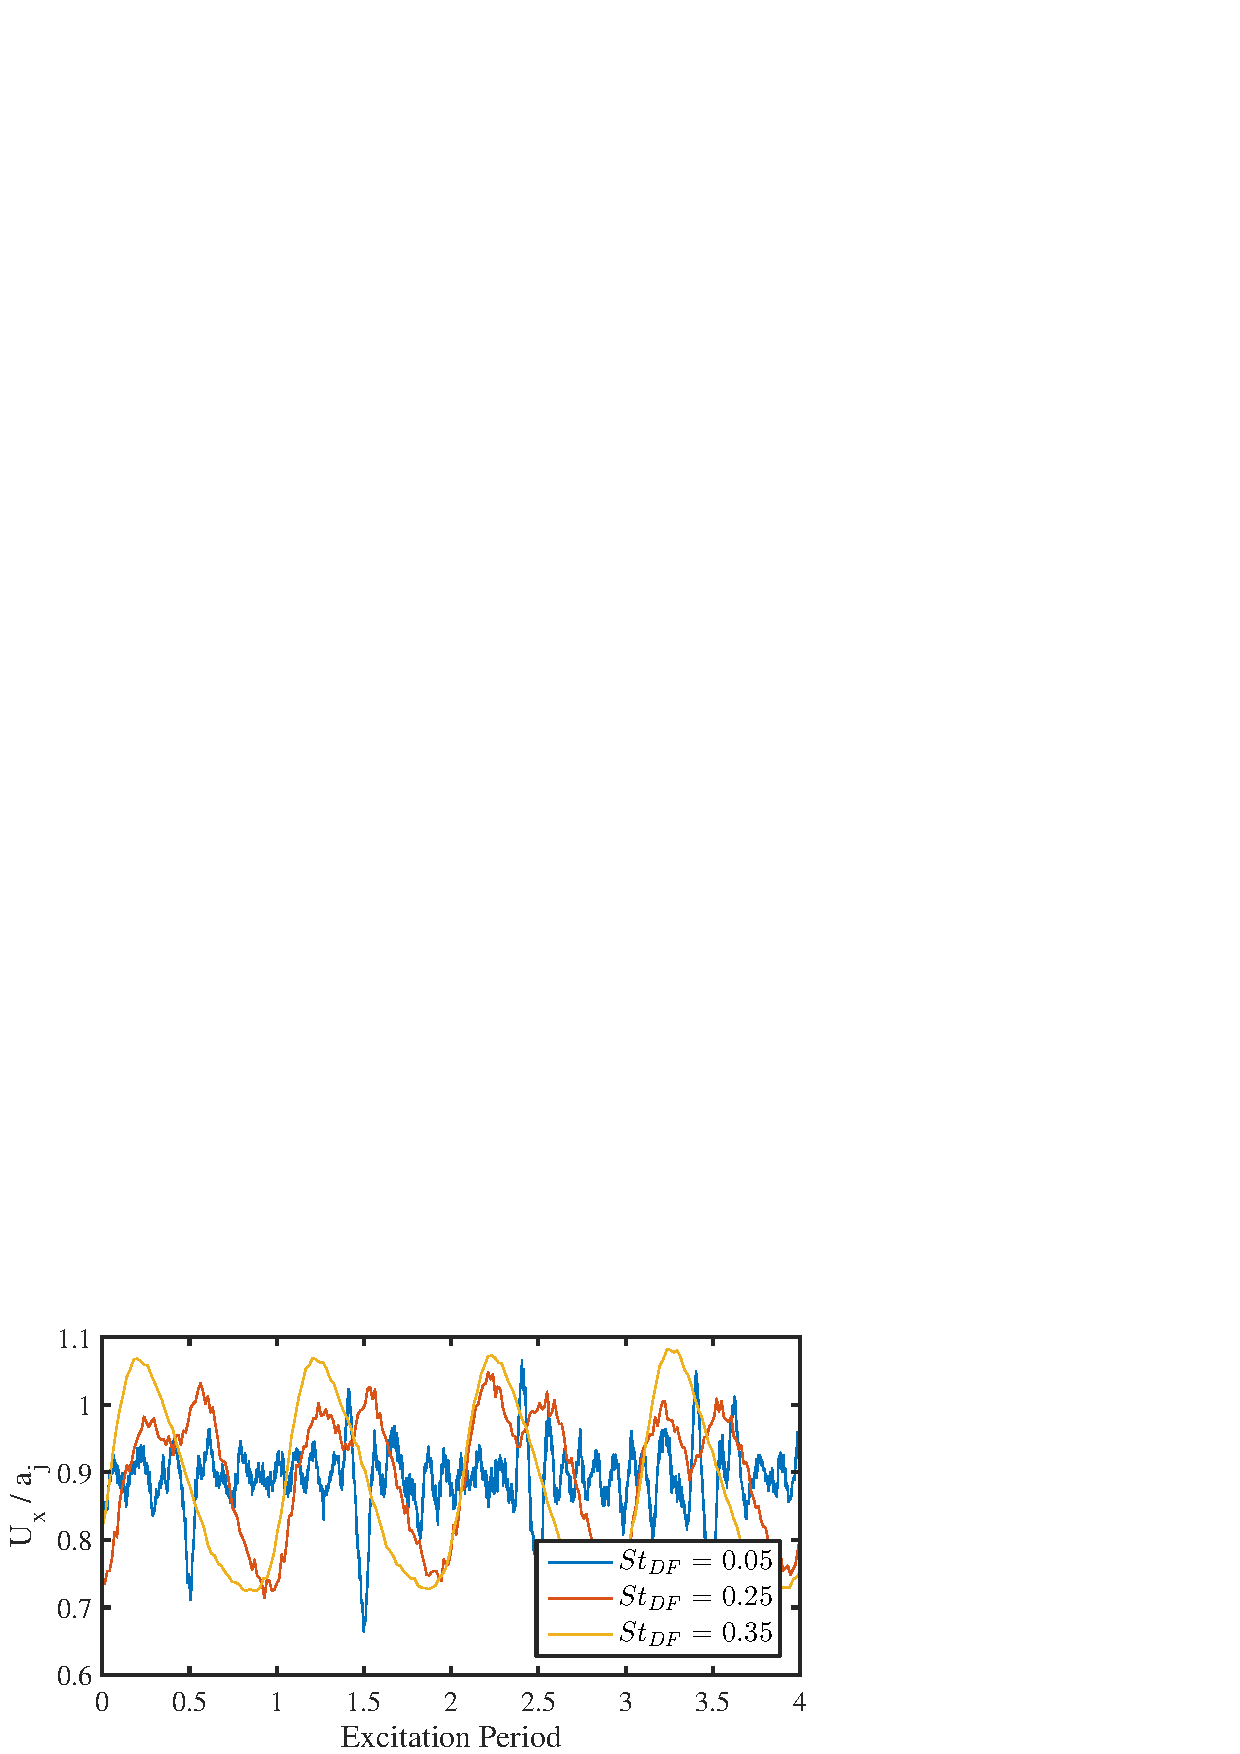
\includegraphics[width=3.5in]{Figures/ch4_centerline_mach_temporal.png} \\
	%		\caption{}
	%		\label{fig:ch4_centerlinemach_temporal}
	%	\end{subfigure}\\
	%	\begin{subfigure}{1\textwidth}
	%		\centering
	\includegraphics[width=3.5in]{Figures/ch4_rawUx_acceleration.png}
	%		\caption{}
	\label{fig:ch4_St005_rawUx_snapshot}
	%	\end{subfigure}
	\caption{Fluctuations associated with the passage of large-scale structures in the axial velocity along the jet centerline at $x/D = 4$ (a) and an arbitrary raw PIV snapshot displaying similar behavior for the $St_{DF}  = 0.05$ jet(b).}
\end{figure}

\subsection{Coherent Structure Merging}
In the simulated subsonic shear layer of \citet{Wei2006}, optimized control for noise mitigation using generalized actuation was implemented using the adjoint perturbation method.
The methodology was able to affect a significant reduction in the emitted noise, though the exact mechanism by which this was accomplished was not immediately clear, even in this highly simplified flow (two-dimensional shear layer).
In \citet{Cavalieri2010b} the same numerical database was investigated with a specific focus on identifying intermittent events related to the noise generation process.
There it was found that the control achieved the majority of the sound reduction by suppressing a single triple vortex interaction, thereby regularizing the flow and preventing the generation of high-amplitude peaks in the acoustic field.
The results of \citet{Kibens1980} also identified vortex merging as a prominent noise source in a (low) subsonic jet.
With this in mind, the evolution of the vortices in the periodically excited jets was analyzed.

\fig{fig:ch4_period_structure_disintegration} illustrates a complete excitation period for the $St_{DF} = 0.25$ excited jet; as before the velocity fields were smoothed prior to computation of the swirling strength, and the results have been phase-averaged over roughly 150 phases.
Previous analysis of the near-field had used two-point correlations between subsequent microphones in order to estimate the convective velocity of the large-scale structures; based on the time-lag for the maximum correlation value, the convective velocity was estimated as $U_c \simeq 0.7 U_j$.
However, the analysis of \citet{Speth2015} in a simulated Mach 0.9 unheated jet found that this method over-predicted the convective velocity; for example, near the end of the potential core two-point correlations in the irrotational near-field produced an estimate of $U_c \simeq 0.67 U_j$ whereas correlations in the \textit{flow}-field produced an estimate of $U_c \simeq 0.64 U_j$.
Essentially, the energy of the acoustic field in the irrotational near-field though small, is non-trivial, and as a result the much higher propagation velocity for the acoustic energy skews the convective velocity estimate to slightly higher values.
By using only the hydrodynamic component of the near-field (produced by the wavelet decomposition of \citet{Crawley2016}), the convective velocity was estimated as $U_c \simeq 0.54 U_j$ near the nozzle exit and $U_c \simeq 0.65 U_j$ near the end of the potential core.
Based on these values, the vortex spacing is expected to be $\simeq 2.6D$ near the end of the potential core.
\begin{figure}
	\centering
	\includegraphics[width=4in]{Figures/ch4_St025_lambda.png}
	\caption{Evolution of the periodic vortex ring ($St_{DF}=0.25$), as visualized using swirling strength. One complete actuation period is shown.}
	\label{fig:ch4_period_structure_disintegration}
\end{figure}

As expected, the excitation produces a periodic roll-up of large-scale structures which, in the downstream region near the end of the potential core, roughly match with the vortex spacing for this frequency (see frame 1 in \fig{fig:ch4_period_structure_disintegration}).
However, in the upstream region ($x/D < 2$) the vortex spacing halves - the LAFPA excitation is in fact producing structures with a frequency associated with the most unstable shear layer frequency, which is significantly higher than the jet column mode frequency.
While this is the first time that this behavior has been observed at the GDTL, it is not terribly surprising if the specifics of LAFPA actuation are considered with respect to the well-known shear layer instability characteristics.
Unlike many other actuators used previously for flow control, the perturbation generated by the LAFPAs is non-sinusoidal and comprised of many higher harmonics than just the fundamental excitation frequency.
These higher harmonics couple to the flow and excite the shear layer instability, which is most unstable at frequencies much higher than the excitation frequencies used in this work.
Therefore, the structures initially formed by the excitation are going to be associated with harmonics of the excitation frequency.
Hence, it is only after merging (or successive mergings) that the passage frequency of the large-scale structures is going to match the fundamental excitation frequency.

In frame 2, the two structures at $x/D = 1$ are beginning to merge.
The trailing structure is inducted inside the preceding structure, and by $x/D \simeq 3$ the merging process is complete.
As the resultant structure convects downstream, the beginning of the breakdown of the vortex is witnessed near $x/D \simeq 4$, similar to the results of the impulsively excited vortex ring and an acceleration of the centerline velocity to slightly supersonic speeds is also observed (\fig{fig:ch4_centerlinemach_temporal}).
Here however, a secondary interaction between structures appears to be occurring, most visibly in frames 5--7. 
Depending on how exactly the coherent vortices are visualized, it appears that a second merging process is commencing here, however the vortices disintegrate before the trailing vortices can be inducted into the first. 
As the vortex at $x/D \simeq 4.5$ is breaking down, the trailing vortex breaks down as well, in fact much more abruptly than the leading vortex; the appearance of structures now matches the excitation frequency.
As the cycle is repeated (beginning again at frame 1), these two vortices (or more accurately, the less coherent, higher-order remnants of them) are no longer individually distinguishable.

Recall that the far-field response of the jet to periodic excitation at $St_{DF}=0.35$ could not be reproduced accurately using a linear superposition of the impulse response.
The vortex dynamics that this excitation frequency produces may thus serve as an insightful contrast for understanding the noise generation phenomena.
A complete excitation cycle for $St_{DF}=0.35$ has been visualized in \fig{fig:ch4_St035_structure_disintegration}.
In this case, two merging processes are now clearly evident.
The first begins just downstream of the nozzle exit, and completes by $x/D \simeq 1.5$; the second begins at $x/D \simeq 2$ and completes relatively quickly, at $x/D \simeq 3$.
It is after this second merging process that the structure spacing now matches the expected wavelength for this excitation frequency ($\lambda \simeq 1.75D$).
As with the lower frequency excitation cases just examined, the dominant vortex (which matches the excitation frequency) undergoes a disintegration beginning around $x/D \simeq 4$.
What is particularly noteworthy here though, is that the disintegration is more rapid for the $St_{DF}=0.05$ and $0.25$ cases than the $St_{DF}=0.35$ case.
In this case, the coherent structure, though severely weakened, is distinguishable over the background noise even downstream of $x/D = 6$.
As with the other excitation frequencies, the core fluid accelerates to supersonic velocities as the large-scale structures pass through the end of the potential core.
\begin{figure}
	\centering
	\includegraphics[width=4in]{Figures/ch4_St035_lambda_evolution.png}
	\caption{Evolution of the periodic vortex ring ($St_{DF}=0.35$), as visualized using swirling strength. One complete actuation period is shown.}
	\label{fig:ch4_St035_structure_disintegration}
\end{figure}

Clearly (and unsurprisingly), the vortex interactions in the periodically-excited jets are far more complex than the impulsively excited jet.
However, as was seen both in terms of the far-field response (\fig{fig:ch3_farfield}) as well as the acoustic source region estimated from the decomposed near-field (\fig{fig:ch3_xcorrOA}), the acoustic fields for $St_{DF}=0.05$ and $St_{DF}=0.25$ show remarkable similarity, at least at angles close to the jet axis.
Therefore, this implies that for this excitation range, the added complexity of the periodic excitation (harmonic structures, vortex merging) are not the primary drivers for noise emission (though they may still play a role).
The consistent, rapid breakdown of the LAFPA-induced structures near $x/D \simeq 4$ and accompanying fluid acceleration in both excited jets appears to be the dominant noise source. 
In contrast, the far-field acoustic response to excitation at $St_{DF}=0.35$ is not accurately reproduced by a linear superposition of the impulse response of the jet.
Analysis of the vortex dynamics demonstrates multiple merging processes occurring for this excitation frequency, and though the dominant vortex breaks down at $x/D \simeq 4$, this process is far less dramatic than in the lower-frequency excitation cases.
In this case, the merging process may in fact be a significant factor in the noise generation process.
In order to more conclusively link this behavior to the noise emission directly, in \sect{sect:source} the aeroacoustic source term will be calculated from the estimated time-resolved velocity fields using a simplified form of Lighthill's acoustic analogy.